\numberedsection{RF5.2 Visualizar relación}

\subsection*{Descripción}
Permite a los usuarios visualizar las relaciones que tienen los distintos productos.\par
\vspace{0.15cm}

\textbf{Pre-condición}\par
El usuario ha iniciado sesión en su cuenta en Mini PIM.\par
\vspace{0.15cm}

\textbf{Post-condición}
\begin{itemize}
    \item Caso de éxito: El sistema muestra la lista de relaciones.
    \item Caso mínimo: El sistema notifica al usuario el resultado de la acción de visualización de relaciones: exitosa o fallida.
\end{itemize}

\textbf{Prioridad: }
Alta
\vspace{0.15cm}

\textbf{Autor: }
Pablo Ortega Serapio\par
\vspace{0.15cm}

\textbf{Control de cambios: } Versión 1: Definición del caso de uso

\numberedsubsection{Escenario principal}
\begin{enumerate}
    \item El usuario ha iniciado sesión con su cuenta de usuario correspondiente.
    \item El usuario accede a la sección de \enquote{Productos}.
    \item El usuario selecciona un producto.
    \item El sistema muestra los detalles del producto.
    \item El sistema muestra en la parte inferior las relaciones en las que está incluido el producto.
    \item El usuario selecciona una relación.
    \item El sistema muestra la lista de productos pertenecientes a esa relación asociados al producto previamente seleccionado.
\end{enumerate}

\numberedsubsection{Escenarios alternativos}
\begin{description}

    \item[3.a] No hay ningún producto creado.
    \begin{enumerate}
        \item[3.a.1] Al no haber ningún producto creado no se puede visualizar las relaciones, se da la opción de crear producto.
    \end{enumerate}

    \item[5.a.] El sistema detecta que no existen relaciones.
    \begin{enumerate}
        \item[5.a.1] El sistema muestra una lista vacía.
    \end{enumerate}

    \item[5.b.] El sistema detecta que el producto no pertenece a ninguna relación.
    \begin{enumerate}
        \item[5.b.1] El sistema muestra una lista vacía.
    \end{enumerate}

\end{description}

\numberedsubsection{Casos de Prueba}
\underline{Escenario: Principal}\par
\vspace{0.15cm}
\textbf{Dado} que he iniciado sesión con mi cuenta de usuario correspondiente,\par
\textbf{Y} estoy en el apartado de \enquote{Productos},\par
\textbf{Cuando} selecciono un producto,\par
\textbf{Y} en los detalles del producto selecciono la relación deseada,\par
\textbf{Entonces} el sistema muestra la lista de productos pertenecientes a esa relación asociados al producto previamente seleccionado.\par

\vspace{0.20cm}

\underline{Escenario: Alternativo 3.a (no hay un producto creado)}\par
\vspace{0.15cm}
\textbf{Dado} que he iniciado sesión con mi cuenta de usuario correspondiente,\par
\textbf{Y} estoy en el apartado de \enquote{Relaciones},\par
\textbf{Y} no hay ningún producto creado,\par
\textbf{Entonces} el sistema muestra la opción de crear producto.\par

\vspace{0.20cm}

\underline{Escenario: Alternativo 5.a (no hay relaciones creadas)}\par
\vspace{0.15cm}
\textbf{Dado} que he iniciado sesión con mi cuenta de usuario correspondiente,\par
\textbf{Y} estoy en el apartado de \enquote{Productos},\par
\textbf{Cuando} selecciono un producto,\par
\textbf{Y} no existen relaciones en el sistema,\par
\textbf{Entonces} el sistema muestra una lista vacía.\par

\vspace{0.20cm}

\underline{Escenario: Alternativo 5.b (producto sin relación asociada)}\par
\vspace{0.15cm}
\textbf{Dado} que he iniciado sesión con mi cuenta de usuario correspondiente,\par
\textbf{Y} estoy en el apartado de producto,\par
\textbf{Cuando} selecciono un producto,\par
\textbf{Y} no está relacionado con ningún producto,\par
\textbf{Entonces} el sistema muestra una lista vacía.\par

\vspace{0.20cm}

\numberedsubsection{Bocetos (por hacer)}
\begin{figure}[H]
    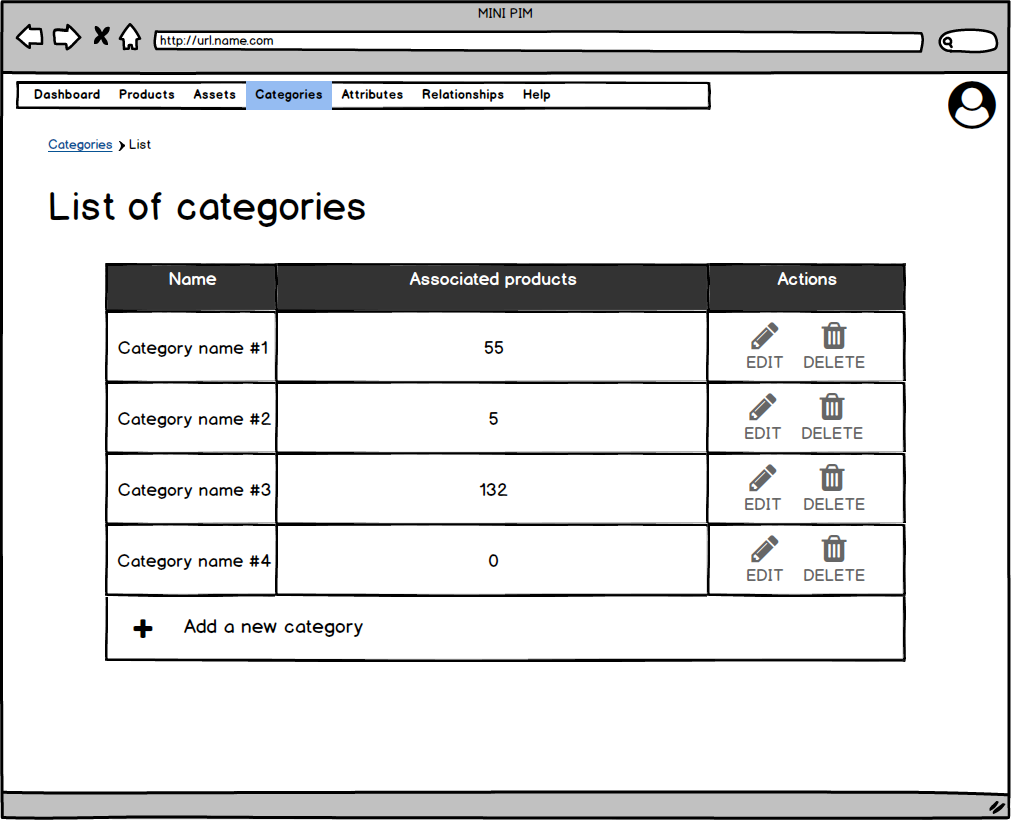
\includegraphics[width=1\linewidth]{assets/mockups/RF4.2_1.png}
    \caption{Visualización de relaciones}
   \end{figure}
\vspace{1.0cm}

\begin{figure}[H]
    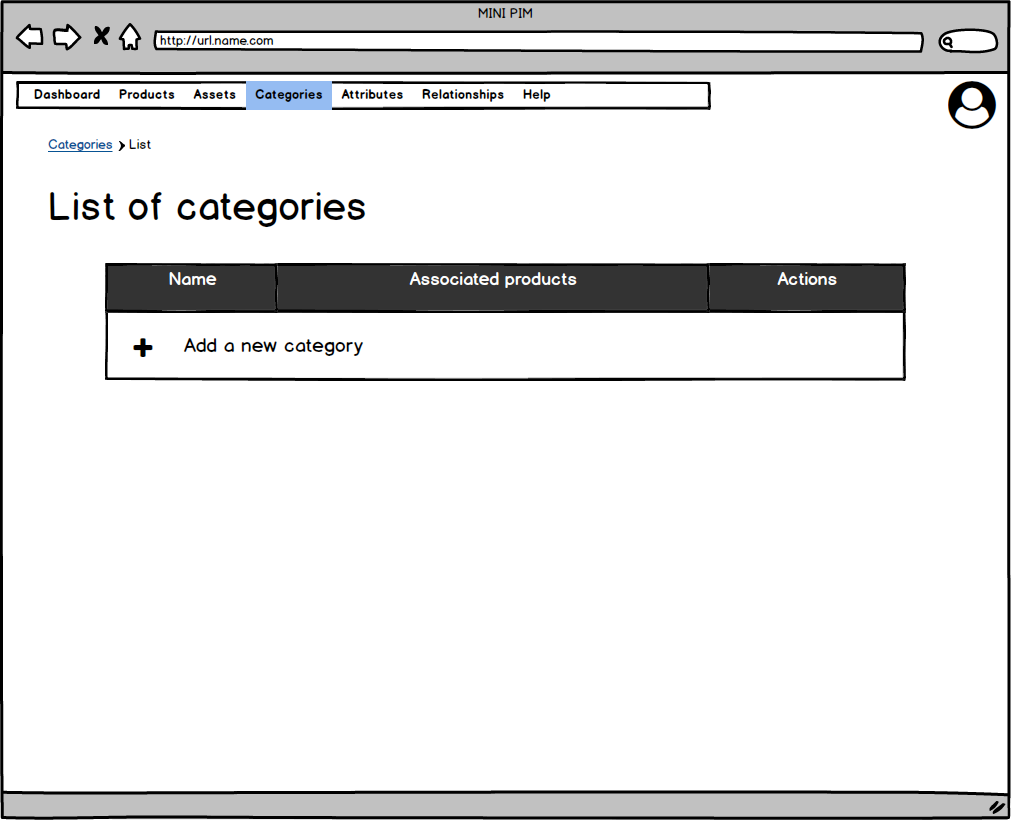
\includegraphics[width=1\linewidth]{assets/mockups/RF4.2_2.png}
    \caption{Visualización de lista vacía}
   \end{figure}
\vspace{1.0cm}

\newpage % Muestra el diagrama de secuencias en una nueva página

\numberedsubsection{Diagrama de Secuencia (por hacer)}
\begin{figure}[H]
    
\includegraphics[width=1\linewidth]{assets/umaLogo.png}
    \caption{Escenario principal para crear el Informe de Cuenta}
   \end{figure}
\vspace{1.0cm}

\newpage % Inicia en una nueva página otro caso de uso